\documentclass{article}
\usepackage{amsmath}
\usepackage{graphicx}
\graphicspath{ {./img/} }

\usepackage{breqn}

\begin{document}
\section{Step method}
\begin{figure}[!ht]
    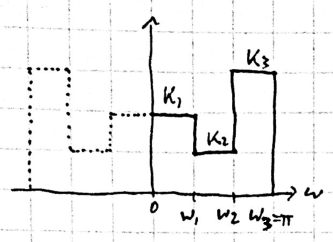
\includegraphics{step}
\end{figure}
\subsection{Ideal non causal}
\begin{equation}
\begin{aligned}
    h_{INC}\left(m\right) = {} & \frac{1}{m\pi}\Bigl[\left(K_1-K_2\right)\sin\left(m\omega_1\right) \\
    & {} + \left(K_2-K_3\right)\sin\left(m\omega_2\right) \\
    & {} + \left(K_3-0\right)\sin\left(m\omega_3\right)\Bigr]
\end{aligned}
\end{equation}

For $m = 0$, use L'Hôpital's rule:
\begin{equation}
\begin{aligned}
    h_{INC}\left(0\right) = {} & \frac{1}{\pi}\Bigl[\left(K_1-K_2\right)\omega_1\cos\left(0\cdot\omega_1\right) \\
    & {} + \left(K_2-K_3\right)\omega_2\cos\left(0\cdot\omega_2\right) \\
    & {} + \left(K_3-0\right)\omega_3\cos\left(0\cdot\omega_3\right)\Bigr]
\end{aligned}
\end{equation}

\begin{equation}
\begin{aligned}
    h_{INC}\left(0\right) = {} & \frac{1}{\pi}\Bigl[\left(K_1-K_2\right)\omega_1 \\
    & {} + \left(K_2-K_3\right)\omega_2 \\
    & {} + \left(K_3-0\right)\omega_3\Bigr]
\end{aligned}
\end{equation}

\subsection{Causal}
\begin{equation}
\begin{aligned}
    h_C\left(n\right) = {} & \frac{1}{\left(n-\frac{N}{2}\right)\pi}\Biggl[\left(K_1-K_2\right)\sin\left(\omega_1\left[n-\frac{N}{2}\right]\right) \\
    & {} + \left(K_2-K_3\right)\sin\left(\omega_2\left[n-\frac{N}{2}\right]\right) \\
    & {} + \left(K_3-0\right)\sin\left(\omega_3\left[n-\frac{N}{2}\right]\right)\Biggr]
\end{aligned}
\end{equation}

$N$ must be even

\subsection{Rectangular window (sinc filter)}
With just a single step $K$, we get a rectangular window and we can simplify the formula to:
\begin{equation}
    h_C\left(n\right) = \frac{1}{\left(n-\frac{N}{2}\right)\pi}\Biggl[K\sin\left(\omega\left[n-\frac{N}{2}\right]\right)\Biggr]
\end{equation}

Considering that $\omega = 2 \pi f$, we get:
\begin{equation}
    h_C\left(n\right) = \frac{1}{\left(n-\frac{N}{2}\right)\pi}\Biggl[K\sin\left(2 \pi f \left[n-\frac{N}{2}\right]\right)\Biggr]
\end{equation}
\begin{equation}
    h_C\left(n\right) = \frac{K\sin\left(2 \pi f \left[n-\frac{N}{2}\right]\right)}{\left(n-\frac{N}{2}\right)\pi}
\end{equation}
\begin{equation}
    h_C\left(n\right) = \frac{2 K f \sin\left(2 \pi f \left[n-\frac{N}{2}\right]\right)}{2 \pi f \left(n-\frac{N}{2}\right)}
\end{equation}
\begin{equation}
    h_C\left(n\right) = 2 K f ~ \text{sinc} \left(2 f \left[n-\frac{N}{2}\right]\right)
\end{equation}

where $\text{sinc}\left(x\right)$ is the normalized sinc function:
\begin{equation}
    \text{sinc} \left(x\right) = \frac{\sin\left(\pi x\right)}{\pi x}
\end{equation}

Assuming we want $K=1$, and say $t=\left[n-\frac{N}{2}\right]$, we can rewrite it as:
\begin{equation}
    h_C\left(n\right) = 2f ~ \text{sinc} \left(2ft\right)
\end{equation}

which represents a sinc filter.


\section{Kaiser window}
\begin{figure}[!ht]
    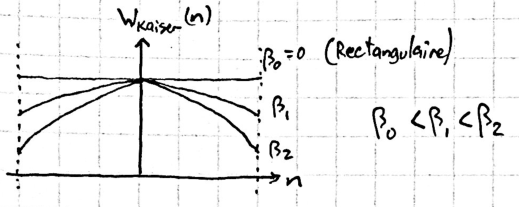
\includegraphics{kaiser-window}
\end{figure}
\subsection{Modified Bessel function of order 0}
\begin{equation}
    I_0\left(x\right) = \sum_{k=0}^{\infty}\frac{\left(\frac{x^2}{4}\right)^k}{\left(k!\right)^2}
\end{equation}

\subsection{Causal window}
\begin{equation}
    W_{K_{C}}\left(n\right) = \frac{I_o\left(\beta\sqrt{1-\left[\frac{n-\frac{N}{2}}{\frac{N}{2}}\right]^2}\right)}{I_o\left(\beta\right)}
\end{equation}

\subsection{Non causal window}
\begin{equation}
    W_{K_{NC}}\left(m\right) = \frac{I_o\left(\beta\sqrt{1-\left[\frac{m}{M}\right]^2}\right)}{I_o\left(\beta\right)}
\end{equation}

\section{Kaiser filter}
\begin{figure}[!ht]
    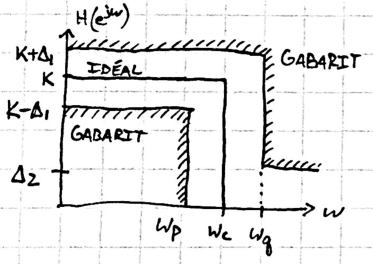
\includegraphics{kaiser-filter}
\end{figure}

\subsection{Parameters}
$K$: passband gain \\
$\Delta_1$: passband ripple \\
$\Delta_2$: stopband attenuation \\
$\omega_q$: transition start pulsation \\
$\omega_p$: transition end pulsation \\
$\Delta\omega$: transition band \\
$\omega_c$: cutoff pulsation

\subsection{Method}
\begin{equation}
    \delta_1 = \frac{\Delta_1}{K}
\end{equation}
\begin{equation}
    \delta_2 = \frac{\Delta_2}{K}
\end{equation}
\begin{equation}
    \delta = \min\left(\delta_1, \delta_2\right)
\end{equation}
\begin{equation}
    \Delta_\omega = \omega_q - \omega_p
\end{equation}
\begin{equation}
    \omega_c = \frac{\omega_q + \omega_p}{2}
\end{equation}
\begin{equation}
    A = -20\log\left(\delta\right)
\end{equation}

\subsection{Order}
\begin{equation}
    N =
    \begin{cases}
        \frac{A-7.95}{2.285\Delta\omega}, & A \geq 21 \\
        \frac{5.79}{\Delta\omega}, & A < 21
    \end{cases}
\end{equation}

$N$ must be even

\subsection{Factor}
\begin{equation}
    \beta =
    \begin{cases}
        0.1102\left(A-8.7\right), & A > 50 \\
        0.5842\left(A-21\right)^{0.4}+0.07886\left(A-21\right), & 21 \leq A \leq 50 \\
        0, & A < 21
    \end{cases}
\end{equation}

\subsection{Windowed filter}
\begin{equation}
    h_{CK}\left(n\right) = h_{C_{REC}}\left(n\right) \cdot W_{K_C}\left(n\right)
\end{equation}

\end{document}
